\documentclass{beamer}
\usepackage{minted}
\usepackage{epigraph}
\usepackage{subfig}
\usepackage{pgfplots}
\usepackage{tikz}
\usepackage{color, colortbl}

\usetheme{focus}

\definecolor{orangered}{rgb}{1,0.45, 0}

\title{Shell Linux \& BASH scripting}
\subtitle{Tutorato Sistemi Operativi}
\author{Davide Carnemolla}
\titlegraphic{
\includegraphics[scale=0.13]{images/penguin2.pdf}}
\institute{Dipartimento di Matematica e Informatica \\ Università di Catania}
\date{2022/2023}

\begin{document}
    \begin{frame}
        \maketitle
    \end{frame}

    \begin{frame}{> whoami}
        
    \end{frame}
    
    \section{Shell Linux}

    \begin{frame}{La Shell}
        \begin{columns}[t, onlytextwidth]
            \column{0.2\textwidth}
                \centering
                
\includegraphics[height=2.5cm, keepaspectratio]{images/user.pdf}

            \column{0.2\textwidth}
                \centering
                
\includegraphics[height=2cm, keepaspectratio]{images/rightarrow.pdf}
            
            \column{0.2\textwidth}
                \centering
                
\includegraphics[height=2.5cm,keepaspectratio]{images/terminal.pdf}

            \column{0.2\textwidth}
                \centering
                
\includegraphics[height=2cm, keepaspectratio]{images/rightarrow.pdf}

            \column{0.2\textwidth}
                \centering
                
\includegraphics[height=2.5cm, keepaspectratio]{images/linux.pdf}
        \end{columns}
    \end{frame}

    \begin{frame}{Il filesystem}
        \centering
        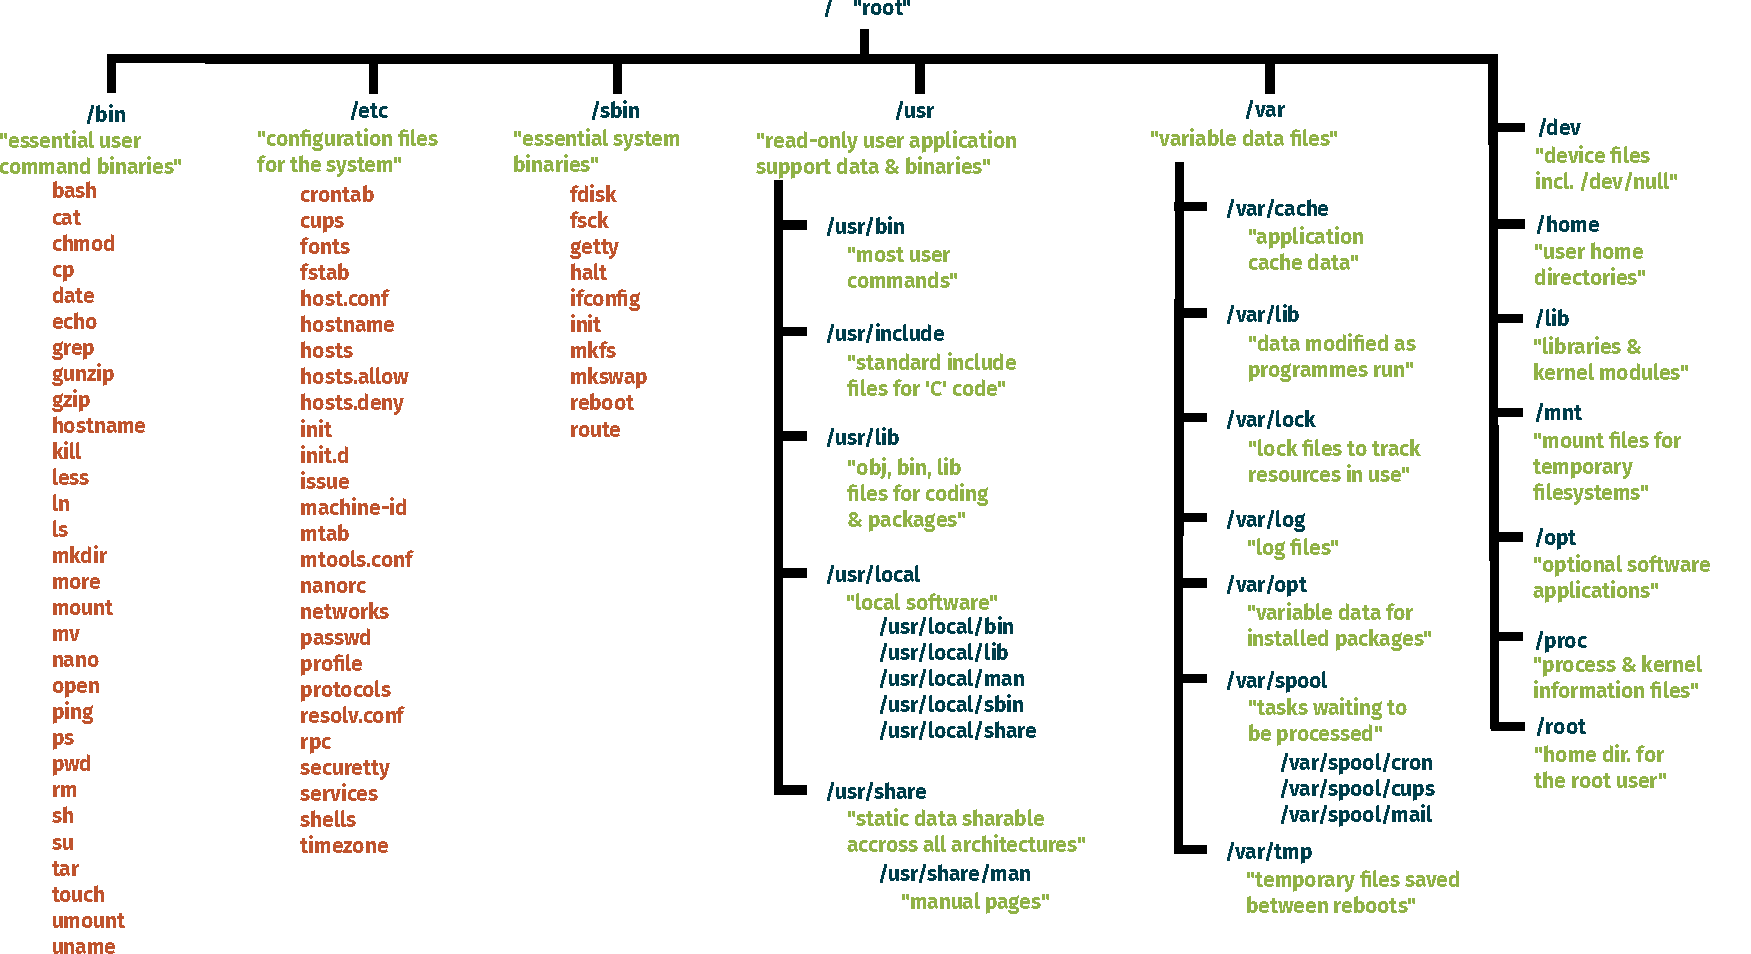
\includegraphics[height=6cm, keepaspectratio]{images/unix-fs.pdf}
    \end{frame}

    \begin{frame}{I Path}
        \centering
        
\includegraphics[height=2cm, keepaspectratio]{images/path.pdf}
        \vspace{0.5cm}
        \begin{block}{Path assoluto}
            Il \textbf{percorso assoluto} di un file è il percorso
            che va dalla radice del filesystem allo stesso.
        \end{block}

        \begin{block}{Path relativo}
            Fissando logicamente una particolare directory (in genere quella corrente) è possibile identificare un file attraverso il
            \textbf{percorso relativo} che va da tale directory ad esso.
        \end{block}
    \end{frame}

    \begin{frame}{I Path}
        \begin{alertblock}{Nota}
            Il percorso assoluto di un file è il suo percorso relativo rispetto
            alla root.
        \end{alertblock}

        \begin{exampleblock}{Esempio}
            \textbf{Directory corrente}: \texttt{/home/}

            \textbf{Path assoluto}: \texttt{/home/davide/file.txt}

            \textbf{Path relativo}: \texttt{davide/file.txt}
        \end{exampleblock}

        \begin{block}{Cartelle virtuali}
            \begin{itemize}
                \item la cartella \texttt{.} indica la cartella stessa
                \item la cartella \texttt{..} indica la cartella genitore (utile per navigare il filesystem)
            \end{itemize}
        \end{block}
    \end{frame}

    \begin{frame}{Path: file di dispositivo}
        In ambiente UNIX esistono dei file speciali chiamati file di dispositivo:
        identificano una particolare periferica del sistema ed attraverso questo è possibile interagire con tale periferica. \\
        \vspace{0.25cm}
        \begin{columns}[t, onlytextwidth]
            \column{0.5\textwidth}
                \centering
                
\includegraphics[height=1.5cm, keepaspectratio]{images/char.pdf}
                
                \textbf{A caratteri}

            \column{0.5\textwidth}
                \centering
                
\includegraphics[height=1.5cm, keepaspectratio]{images/block.pdf}
                
                \textbf{A blocchi}
        \end{columns}

        \vspace{0.25cm}

        \begin{exampleblock}{Esempi}
            \begin{itemize}
                \item \texttt{/dev/sda,/dev/sdb}\dots
                \item \texttt{/dev/sda1,/dev/sda2}\dots
                \item \texttt{/dev/tty1,/dev/tty2}\dots
            \end{itemize}
        \end{exampleblock}
    \end{frame}

    \begin{frame}{Path: file di dispositivo speciali}
    \end{frame}

    \begin{frame}{Mount: quando voglio più spazio}
        \centering
        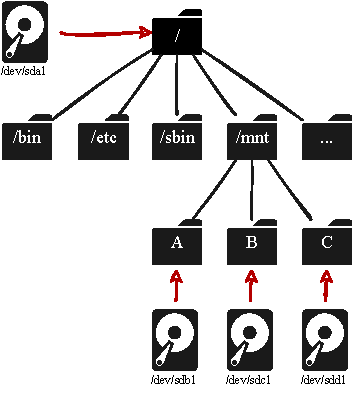
\includegraphics[height=7.5cm, keepaspectratio]{images/mountpoint.pdf}
    \end{frame}

    \begin{frame}{Hello Shell}
        \begin{exampleblock}{}
            \texttt{\$ echo "Hello shell"}
        \end{exampleblock}

        \begin{itemize}
            \item \textbf{echo} rappresenta il comando
            \item \textbf{"Hello world"} rappresenta un parametro per il comando
        \end{itemize}

        \begin{block}{Parametri}
            Tipicamente un comando può richiedere dei parametri
            
            \vspace{0.5cm}

            \begin{columns}[t, onlytextwidth]
                \column{0.33\textwidth}
                    \centering
                    
\includegraphics[height=1cm, keepaspectratio]{images/file.pdf}
                    
                    \textbf{File}
    
                \column{0.33\textwidth}
                    \centering
                    
\includegraphics[height=1cm, keepaspectratio]{images/input-data.pdf}
                    
                    \textbf{Dati}
                \column{0.33\textwidth}
                    \centering
                    
\includegraphics[height=1cm, keepaspectratio]{images/options.pdf}
                    
                    \textbf{Opzioni}
            \end{columns}

            \vspace{0.5cm}
        \end{block}
    \end{frame}

    \begin{frame}{Comandi utili}
        \begin{columns}[t, onlytextwidth]
            \column{0.33\textwidth}
                \centering
                \Huge \textbf{CTRL + C}
                
                \vspace{0.2cm}
                
                \normalsize \textit{``No maria, io esco''}
            \column{0.33\textwidth}
                \centering
                \Huge \textbf{CTRL + S}

                \vspace{0.2cm}

                \normalsize \textit{``Finisco di mangiare la peperonata e scendo! ''}
            \column{0.33\textwidth}
                \centering
                \Huge \textbf{CTRL + Q}

                \vspace{0.2cm}

                \normalsize \textit{``Ok ho digerito: possiamo riprendere.''}
        \end{columns}
    \end{frame}

    \begin{frame}{Comandi utili}
        \centering
        
\includegraphics[height=4cm,keepaspectratio]{images/spongebob-crying.png}

        \Large \textit{``Non riesco a fare copia e incolla''}
        
        \vspace{1cm}

        \begin{columns}[t, onlytextwidth]
            \column{0.5\textwidth}
                \centering
                \huge \textbf{CTRL+SHIFT+C}
            \column{0.5\textwidth}
                \centering
                \huge \textbf{CTRL+SHIFT+S}
        \end{columns}
    \end{frame}

    \begin{frame}{Hello man}
        \begin{columns}[t, onlytextwidth]
            \column{0.33\textwidth}
                \centering
                
\includegraphics[height=2cm]{images/search.pdf}

                \vspace{0.2cm}

                \textit{apropos stringa}
            \column{0.33\textwidth}
                \centering
                
\includegraphics[height=2cm]{images/whatis.pdf}

                \vspace{0.2cm}

                \textit{whatis stringa}
            \column{0.33\textwidth}
                \centering
                
\includegraphics[height=2cm]{images/man.pdf}

                \vspace{0.2cm}

                \textit{man stringa}
        \end{columns}
    \end{frame}

    \begin{frame}{Filesystem: ls}
        \begin{block}{ls}
            Sintassi: \texttt{\textbf{ls [-l] [-a] [-R] [pathname\dots]}}

            \begin{itemize}
                \item \texttt{\textbf{-l}}: visualizza informazioni dettagliate
                \item \texttt{\textbf{-a}}: visualizza anche i file nascosti
                \item \texttt{\textbf{-R}}: visualizza il contenuto delle cartelle ricorsivamente
                \item \texttt{\textbf{pathname}}: oggetto del filesystem sul quale visualizzare le informazioni
            \end{itemize}
        \end{block}

        \begin{exampleblock}{Esempio}
            \$ ls /home/davide/script.sh
            
            -rw-r-{}-r-{}- 1 davide davide 967 31 mag 23.05 script.sh
        \end{exampleblock}
    \end{frame}

    \begin{frame}{Permessi di accesso}
        Nei sistemi Unix ogni file possiede dei permessi di accesso.

        In principali sono:
        \begin{itemize}
            \item \textbf{r}: lettura
            \item \textbf{w}: scrittura
            \item \textbf{x}: esecuzione/attraversamento (directory)
        \end{itemize}

        \vspace{0.5cm}

        Inoltre, il primo carattere è destinato a dei flag speciali:
        \begin{itemize}
            \item \textbf{d}: si tratta di una directory
            \item \textbf{l}: si tratta di un soft link
            \item \textbf{s}: attribuisce al file in esecuzione i privilegi dell'utente cui appartiene (SUID)
        \end{itemize}

        \begin{exampleblock}{Esempio}
            -rw-r-{}-r-{}- 1 davide davide 967 31 mag 23.05 script.sh
        \end{exampleblock}
    \end{frame}

    \begin{frame}{I metacaratteri}
        Per abbreviare il nome di un file da specificare o per specificarne più di uno
        si possono utilizzare i metacaratteri:
        \begin{itemize}
            \item \textbf{*}: rappresenta una qualunque stringa di 0 o più caratteri
            \item \textbf{?}: rappresenta un qualsiasi carattere
            \item \textbf{[]}: singolo carattere tra quelli elencati
            \item \textbf{\{\}}: singola stringa tra quelle elencate
        \end{itemize}
        \begin{exampleblock}{Esempio}
            \$ ls

            esempio2.txt esempio3.txt esempio.txt script.sh scheda.pdf

            \$ ls esempio*.txt

            esempio2.txt esempio3.txt esempio.txt

            \$ ls esempio?.txt

            esempio2.txt esempio3.txt esempio.txt

            \$ ls *.\{txt,pdf\}

            esempio2.txt esempio3.txt esempio.txt scheda.pdf
        \end{exampleblock}
    \end{frame}

    \begin{frame}{Filesystem: cd/pwd}
        \begin{block}{cd}
            Sintassi: \texttt{\textbf{cd [pathname]}}
            
            \begin{itemize}
                \item \textbf{pathname}: nuova directory corrente (assoluto o relativo)
            \end{itemize}

            Il comando ci permette di navigare all'interno del
            filesystem cambiando di volta in volta la directory corrente.
        \end{block}

        \begin{block}{pwd}
            Sintassi: \texttt{\textbf{pwd}}

            Il comando ci permette di ottenere la \textit{present working directory}, ovvero il path assoluto
            della directory in cui ci troviamo.
        \end{block}
    \end{frame}

    \begin{frame}{Filesystem: mkdir/rmdir}
        \begin{block}{mkdir}
            Sintassi: \texttt{\textbf{mkdir [-p] pathname\dots}}

            \begin{itemize}
                \item \texttt{\textbf{-p}}: non restituisce errori se la directory esiste già e crea tutte le directory necessarie per ottenere il path completo
                \item \texttt{\textbf{pathname}}: pathname da creare
            \end{itemize}

            Il comando \textbf{mkdir} crea le directory specificate mediante i parametri.
        \end{block}

        \begin{block}{rmdir}
            Sintassi: \texttt{\textbf{rmdir [-p] pathname\dots}}

            \begin{itemize}
                \item \textbf{-p}: rimuove tutte le directory presenti nel pathname
                \item \textbf{pathname}: directory da eliminare
            \end{itemize}

            Il comando \textbf{rmdir} rimuove una directory vuota dal filesystem.
        \end{block}
    \end{frame}

    \begin{frame}{Filesystem: cp}
        \centering
        
\includegraphics[height=2.5cm, keepaspectratio]{images/spider-man-meme.jpg}

        \begin{block}{cp}
            Sintassi: \texttt{\textbf{cp [-R] [-i] source... dest}}

            \begin{itemize}
                \item \textbf{-R}: copia ricorsivamente il contenuto di una directory
                \item \textbf{-i}: chiede conferma prima di sovrascrivere i file
                \item \textbf{source}: oggetti da copiare
                \item \textbf{dest}: destinazione in cui copiare gli oggetti
            \end{itemize}

            Il comando \textbf{cp} copia i file specificati con \textbf{source} in \textbf{dest}.
        \end{block}
    \end{frame}

    \begin{frame}{Filesystem: rm}
        \centering
        
\includegraphics[height=3cm, keepaspectratio]{images/willy.jpg}

        \begin{block}{rm}
            Sintassi: \texttt{\textbf{rm [-r] [-i] [-f] pathname...}}

            \begin{itemize}
                \item \textbf{-r}: elimina ricorsivamente tutti i file
                \item \textbf{-i}: chiede conferma prima di cancellare ogni file
                \item \textbf{-f}: cancella gli oggetti senza chiedere conferma
                \item \textbf{pathname}: oggetti da eliminare
            \end{itemize}

            Il comando \textbf{rm} elimina tutti i file specificati con i parametri.
        \end{block}
    \end{frame}

    \begin{frame}{}
        \centering
        \Huge \texttt{rm -rf /}
    \end{frame}

    \begin{frame}{Filesystem: mv}
        \centering
        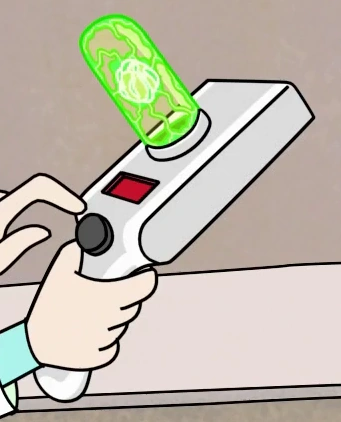
\includegraphics[height=3cm, keepaspectratio]{images/spara-porte.png}

        \begin{block}{mv}
            Sintassi: \texttt{\textbf{mv source... dest}}

            \begin{itemize}
                \item \textbf{source}: file o directory da spostare
                \item \textbf{dest}: file o directory di destinazione
            \end{itemize}

            Il comando \textbf{mv} sposta il file o directory sorgente nella destinazione specificata.
        \end{block}
    \end{frame}

    \begin{frame}{Filesystem: chmod}
        \begin{block}{chmod}
            Sintassi: \texttt{\textbf{chmod [-R] mode [pathname...]}}

            \begin{itemize}
                \item \textbf{-R}: applica i permessi ricorsivamente
                \item \textbf{mode}: nuova maschera dei permessi
                \item \textbf{pathname}: oggetti a cui applicare la nuova maschera
            \end{itemize}

            Il comando \textbf{chmod} permette di cambiare i permessi dei file.
        \end{block}

        \begin{alertblock}{mode: sintassi numerica}
            \texttt{rw-r-{}-{}-{}-{}- $\rightarrow$ 110 100 000 $\rightarrow$ 640}

            \texttt{rwxr-xr-x $\rightarrow$ 111 101 101 $\rightarrow$ 755}
        \end{alertblock}

        \begin{alertblock}{mode: sintassi simbolica}
            \texttt{rw-r-{}-{}-{}-{}- $\leftrightarrow$ u=rw,g=r,o-rwx}
        
            \texttt{rw-rw-rw- $+$ u+x,o-rw $\rightarrow$ rwxrw-{}-{}-{}-}
        \end{alertblock}
    \end{frame}

    \begin{frame}{Filesystem: chown}
        \centering
        
\includegraphics[height=3cm, keepaspectratio]{images/bugs-bunny-capitalist.png}
        \begin{block}{chown}
            Sintassi: \texttt{\textbf{chown [-R] owner[:group] [pathname...]}}

            \begin{itemize}
                \item \texttt{\textbf{-R}}: esegue ricorsivamente le modifiche di proprietà
                \item \texttt{\textbf{owner}}: il nuovo proprietario
                \item \texttt{\textbf{group}}: il nuovo gruppo proprietario
                \item \texttt{\textbf{pathname}}: oggetti a cui vogliamo cambiare la proprietà
            \end{itemize}
        \end{block}
    \end{frame}

    \begin{frame}{}
        \centering
        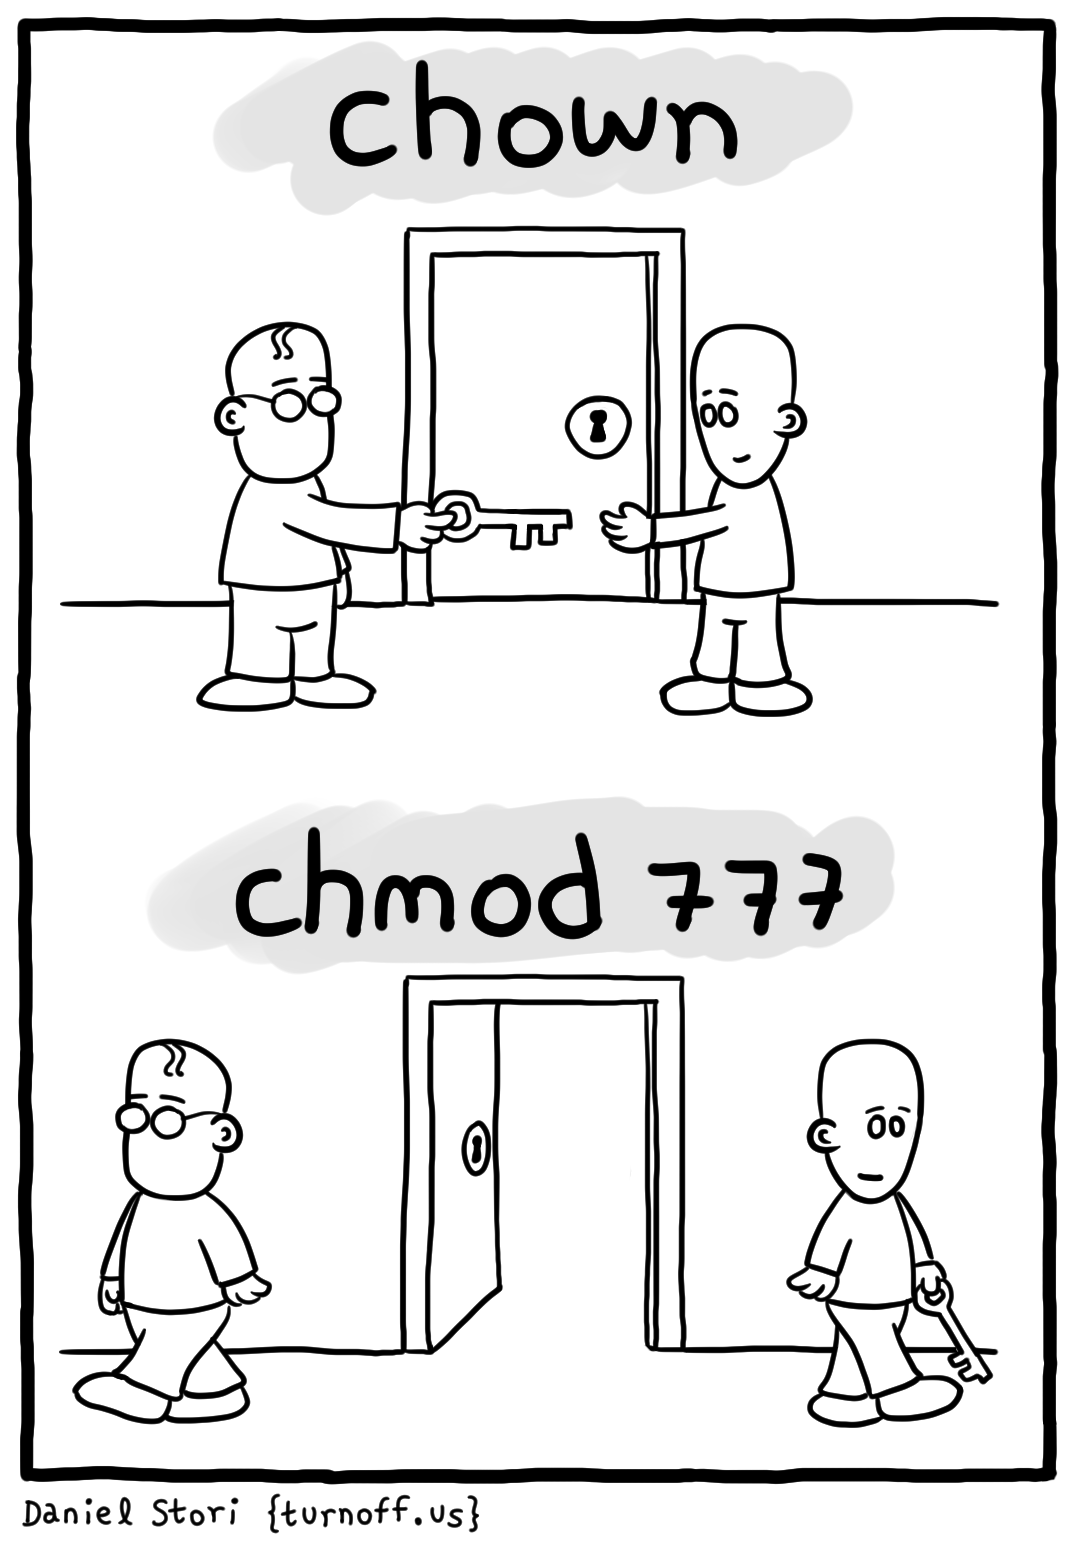
\includegraphics[height=8cm, keepaspectratio]{images/chown-chmod.png}
    \end{frame}

    \begin{frame}{Utenti nei sistemi Unix}
        \begin{columns}[t, onlytextwidth]
            \column{0.33\textwidth}
                \centering
                
\includegraphics[height=2.5cm, keepaspectratio]{images/root.pdf}

                \large \textbf{root}
            \column{0.33\textwidth}
                \centering
                \Huge $\longleftarrow$

                \large sudo
            \column{0.33\textwidth}
                \centering
                
\includegraphics[height=2.5cm, keepaspectratio]{images/user2.pdf}

                \large \textbf{standard user}
        \end{columns}
    \end{frame}

    \begin{frame}{Filesystem: link}
    \end{frame}

    \begin{frame}{Filesystem: ln}
    \end{frame}

    \begin{frame}{Filesystem: find}
    \end{frame}

    \begin{frame}{Redirezione dell'I/O}
    \end{frame}

    \begin{frame}{cat}
        \centering
        
\includegraphics[height=3cm, keepaspectratio]{images/garfield.jpg}

        \begin{block}{cat}
        \end{block}
    \end{frame}

    \begin{frame}{less \& more}
    \end{frame}

    \begin{frame}{echo}
    \end{frame}

    \begin{frame}{grep}
    \end{frame}

    \begin{frame}{Espressioni regolari}
    \end{frame}

    \begin{frame}{Pipeline}
    \end{frame}

    \begin{frame}{wc}
    \end{frame}

    \begin{frame}{sort}
    \end{frame}

    \begin{frame}{Head \& Tail}
    \end{frame}

    \begin{frame}{Tar}
    \end{frame}

    \begin{frame}{Alias}
    \end{frame}

    \begin{frame}{Modalità di esecuzione}
    \end{frame}

    \section{BASH}


    
\end{document}
